
\section{Buildtools}
Because we are in \textbf{Group 6}, we had to read "Overhauling Amd for the '00s: A Case Study of GNU Autotools" for this weeks homework assignment. Listed below are our remarks regarding the paper. These remarks are split in two pieces; structural remarks which talk about how the paper was structured and substantive remarks which comment on the actual contents of the paper. 

\subsection{Structural remarks}
We found that the paper is well-structured: Zadok starts things of with an explanation about the inner workings of autotools and all its inherent tests and dependencies. After that the writer defines what makes an application difficult to port over to a different system. He concludes with a writeup about how the developers of the ''am-utils'' package benefited from rewriting their ''amd'' package to use autotools (renaming the package to 'am-utils' in the process). The author of the paper lets his own experience weigh in as he has personal experience with autotools which in turn enhances the credibility of his opinions and views.

I do however feel that the conclusion of the paper is a bit lacking. Zadok ends on the notion that autotools helped ''am-utils'' to grow, but also points out a fair amount of weak points in the build tools. Even though he plans on developing a toolkit that can judge how complex a software package is, he does not propose any improvements to the autotools themselves. As he is fairly invested in autotools in general I had hoped to see at least some proposals in regards to making the porting of complex code a more consistent and convenient experience. 

\subsection{Substantive remarks}
Reading the paper is a bit of an emotional rollercoaster. First the author starts out by pointing out all the benefits autotools pose over older methods of building applications. For example, he talks about how the automation factor of the buildtools made it so that end users don't need to have in-and-out knowledge of their system anymore and how code became easier to maintain. Then he all of a sudden starts pointing out the problems autotools have according to him. Although we largely agree with the points he makes throughout the paper, we question some of his partial conclusions. To illustrate we'll go over some of these partial conclusions and note our remarks below. 

At some point in the paper Zadok talks about how the tests in autotools are very extensive, but don't cover all the needs of developers. He writes the following:

\begin{quotation}
"The conclusion we draw in this section is that although Autoconf continues to evolve and provide more tests, maintainers of large and complex packages may still have to write 10–30 custom macros. Moreover, some packages will always need a number of static macros, for those features that Autoconf cannot test in a reliable, automated way".
\end{quotation}

As a reader I feel that it is unfair to fault autotools for this 'problem' too much, because this was a problem initially as well. Before autotools were introduced developers and administrators had to jump convoluted hoops in order to port their application to different platforms. Granted, it is supposedly difficult to convert a package to use autotools, but it (should be) worth it in the end as the buildtools make the need for custom macros a lot lower. Because Autoconf out of the box supports a whole slew of pre-created tests, the developers of ''am-utils'' only had to write new tests for a small portion of their code. Table \ref{table:worthlesstable} shows a pretty worthless table.

\begin{table}[H]
	\center
	\begin{tabular}{|c|c|c|}
	\hline 
	\textbf{Amount of lines} & \textbf{C++ constructs} & \textbf{System calls} \\ 
	\hline 
	Bad & Good & Best \\ 
	\hline 
	\end{tabular}
	\caption{This is a worthless table}
	\label{table:worthlesstable}
\end{table}

A substantial part of the paper talks about the complexity of code and the different metrics used to measure this complexity. Even though I am not a software developer I disagree to some extent with the metrics for code complexity posed in the paper. In the first graphs, the number of lines of code is used as a complexity metric. Luckily the writer also takes up other metrics in the latter part of the report. Zadok settles on the metric of the ''amount of CPP constructs per 1000 lines of code''. Although this lets you know something about the overall complexity of the code it is in my opinion unrelated to the portability issues which the author encountered whilst incorporating autotools in ''amd''. 

Namely, the amount of low level system calls which the package has to make made porting the application so difficult. ''am-utils'' makes use of a lot of lowlevel kernel calls which in turn require a lot of custom or static Autoconf tests. The portability of the application is therefore closely related to the amount of system calls an application makes. Even though software like ''gcc'' and ''Binutils'' are much larger applications, they mainly do text-parsing, which usually consists of rather portable code. Even though the code that the application is written in is generally cross-platform, the system calls that the program makes are non-standardized which naturally creates code portability issues. Therefor I think the ''amount of system calls per 1000 lines of code'' defines the complexity for portability better. I may be mistaken, but I feel the writer is talking about different kinds of complexity throughout his paper. 

\begin{quotation}
"The conclusion we draw from our experiences is that large packages can benefit greatly from using autotools such as Autoconf. Autoconf-based packages are easier to maintain, develop, and port to new systems".
\end{quotation}

Even though this statement holds true in most cases, Zadok also states that their ''amd'' package grew in functionality (which took around 60.000 lines of code) after the incorporation of autotools. Therefor I personally think that not only large packages can benefit from autotools as smaller packages could benefit from the enhanced code maintaining functionality as well. They would get the chance to grow faster due to the incorporation of the build tools. 

Lastly, the paper mentions that compiling code with autotools is five times slower than directly building the package due to the different steps the autotools have to take in order to compile a package. It is questionable whether this is still a problem in modern day and age due to the increased speed of processors. Mind you that the tests performed in that paper make use of a \textit{Pentium III processor} with 128MB of RAM. Personally I think that the speed gain from \underline{not} using autotools nowadays is negligible. 

\begin{figure}[H]
	\centering
	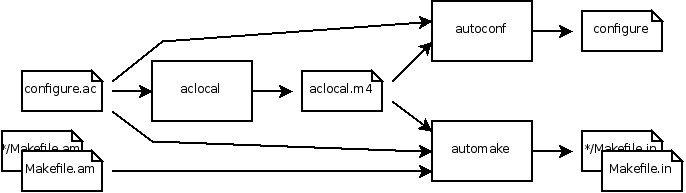
\includegraphics[scale=0.4]{/home/siem/sne-es-latex/img/autotools.png}
	\caption{A totally pointless image}
	\label{fig:pointlessimage}
\end{figure}

Judging from my current knowledge about the subject, I think that autotools have been good for development, and I think it would be hard to argue against that. Zadok encountered that the conversion from ''amd'' to ''am-utils'' was a rather bumpy ride. However, I think that this was largely due to the fact that he tried to incorporate autotooling in the original ''amd'' package. Perhaps if a developer would create an application right now and would incorporate the autotools from the beginning, the overall experience would be a lot smoother. Furthermore, as Zadok states in his paper, ''am-utils'' is unique in the sense that the package requires a large amount of low-level system calls which makes the package portability inherently much more difficult. Also take a look at figure \ref{fig:pointlessimage} below \footnote{Using Autotools. (n.d.). Retrieved September 27, 2015, from https://developer.gnome.org/anjuta-build-tutorial/stable/create-autotools.html.en}.

\subsection{Closing remarks}
We generally agreed on the points posed in the text above. Below are however some extra points points about the paper. 

\emph{\textcolor{red}{Bram ter Borch}}
\begin{quotation}
"In my opinion the paper was fine to read. But it was very detailed in the way he had to work around the shortcomings in the auto tools for his specific application. The examples of his own test scripts do not add anything to the paper. Beside that he introduces a new way to measure complexity. So you are right, he is talking about different ways of complexity."
\end{quotation}
\textit{Bram also writes the following:}

\begin{quotation}
In your document, you write about the speed of compiling. I think it didn't change over time. Zadok is right about his statement. He tested compiling and installing the application before auto tooling and after. When compiling auto tools needs to do a lot of checks. This takes time. And nowadays programs become much larger than 10 years ago. Auto tools contains a lot more tests it needs to work through. Due to the increase of operating systems in my opinion compiling a program is not a lot faster than 10 years ago. Even with the hardware we currently have.
After a short discussion we have agreed to disagree on this point. I personally hold the opinion that the amount of tests hasn't had the same turbulent growth that processors have had. I may however be wrong on this. 

I share you opinion in the advantage of auto tools. It is the way to go. Zadok took a long time to master auto tools, he needed to change his way of programming to fit into the auto tools ways, but in the long run he, and the functionality of the package greatly benefit from the incorporation.
\end{quotation}

\emph{\textcolor{red}{Jeroen Schutrup}}
\begin{quotation}
"I agree with both of you guys arguments. Something that was not clear to me was the fact that am-utils was more complex than amd after they moved to autotools, to be seen in Figure 3. Besides, I wonder how much of a burden the complexity overhead of not having autotools actually was. After they switched to autotools, their codebase decreased from 90k to 60k lines. From there on, they managed to recreate these 30k lines of code they've just saved, almost within one month worth of time. So I wonder how much of an issue the complexity was to them."

With this notion Jeroen highlight the biggest problem I have with this paper: the concept of complexity is very loosely defined throughout the paper. The increase in code however was due to the added functionality. This functionality could be added because it became easier to maintain the codebase after autotools were introduced in the build process. 
\end{quotation}
